\input{../tex/baliky}


%  Nastaví autora, název, datum, skupinu měření apod. (můj vlastní
% příkaz, umožní znovu-použití v dokumentu)
\newcommand{\Author}{Vojtěch Fišer}
\newcommand{\Institute}{FJFI ČVUT v Praze}
\newcommand{\Subject}{Fyzikální praktika 1}
\newcommand{\Group}{2}
\newcommand{\Title}{Úloha číslo \#10 : Interference}
\newcommand{\Date}{20.4.2016}

% Začátek dokumentu - Formátování na výstup
\begin{document}


\setlength{\parindent}{0cm}
\textsf{\textbf{Základy fyzikálního měření II \hfill FJFI ČVUT v Praze}\hspace*{1cm}}\\[0.1cm]
\textsf{\textbf{\large{Úloha 0 \\
			\raggedleft Psaní vzorového protokolu
}}}
\vspace{-0.6cm}
\setlength{\columnsep}{120pt}
\begin{multicols}{2}
	\noindent
	\linebreak
	\begin{tabular}{llll}
		\textsf{Jméno:} & \textsf{\textbf{Křemílek}} & \textsf{Kolega}: & \textsf{Vochomůrka} \\[0.05cm] 
		\textsf{Kruh:} & \textsf{Sobota 19:00} & \textsf{Číslo skup.:} & \textsf{10}  \\[0.05cm]
		\textsf{Měřeno:} & \textsf{1. 1. 1993}  & \textsf{Náročnost\ |\ zábava:} & $\sfrac{0}{10}\;|\;\sfrac{10}{10} $ \\[0.05cm]
		\textsf{Obor:} & \textsf{JČF} & \textsf{Klasifikace:} & 
	\end{tabular}
	\linebreak
	\columnbreak
	\hspace*{0.5cm}
	
\includegraphics[height=2cm]{img/fjfi.pdf}
	\hspace{0.4cm}
	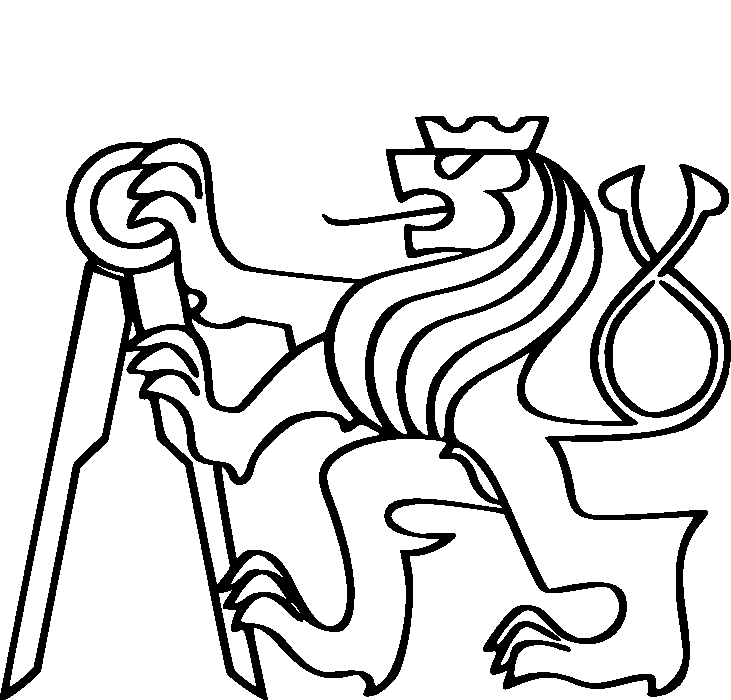
\includegraphics[height=2cm]{img/cvut.pdf}
	\hspace*{0.3cm}
\end{multicols}
\vspace*{-0.1cm}
\hrule
\setlength{\parindent}{0.5cm}


\section{Úkoly} % (fold)
\label{sec:_koly}

  \begin{enumerate}
\item \textbf{DÚ: Ve vztazích \eqref{eq:maxima_mrizka}, \eqref{eq:minima_sterbina} a \eqref{eq:minima_kruh} vyjádřete $\sin \vartheta$ pomocí polohy maxima/minima od středu a uražené dráhy laserového paprsku}
\item Změřte průměr tří nejmenších kruhových otvorů užitím Fraunhoferovy difrakce světla s pomocí měřicího mikroskopu a výsledky srovnejte. Odhadněte chybu měření šířky štěrbiny
mikroskopem. Pro který průměr kruhového otvoru je přesnější měření interferencí a pro který mikroskopem?
\item Změřte 10 různých šířek štěrbiny užitím Fraunhoferovy difrakce světla a srovnejte s hodnotou na mikrometrickém šroubu. Pro jaké šířky štěrbiny je výhodnější měření interferencí a pro jaké mikrometrickým šroubem?
\item Změřte mřížkovou konstantu optické mřížky a srovnejte s hodnotou uvedenou na mřížce.
\item Sestavte Michelsonův interferometr a změřte vlnovou délku laserového svazku.
  \end{enumerate}

\section{Pomůcky} % (fold)
\label{sec:pom_cky}
Železná deska s magnetickými stojánky, He-Ne laser (633 nm, 5 mW), 2 zrcadla na stojánku, optická lavice s jezdci, 2 spojky (+50, +200), rozptylka (-100), sada kruhových otvorů, nastavitelná štěrbina s mikrometrickým šroubem, stojan na mřížku, optická mřížka, stínítko na zdi, stínítko, držák na stínítko a kruhové otvory, pásmové měřidlo (5 m), pravítko 20 cm a 30 cm, měřicí mikroskop, Abbeho kostka, rovinné zrcadlo s mikrometrickým šroubem, rovinné zrcadlo
% section pom_cky (end)
\section{Teorie} % (fold)
\label{sec:teorie}
	Interferencí nazýváme skládání vln z diskrétních zdrojů. Typický příklad interferenčního jevu je youngův dvouštěrbinový experiment. Proti tomu difrakcí nazýváme skládání vln ze zdrojů rozloženáých spojitě.

	\subsection{Babinetův princip} % (fold)	
	\label{sub:babinetův_princip}
		Pomocí Babinetova principu je možno snadno vysvětlit interferenční jevy, kterými se budeme zabývat.

		Babinetův princip tvrdí, že v místě dopadu na neprůstupnou překážku se generuje obrácené elektromagnetické pole. Bod dopadu se tedy také stává zdrojem záření. Z Babinetova principů pak také vyplývá, že difrakční obrazec nějaké konfigurace přepážky je stejný, jako difrakční obrazec jeho plošné inverze.	
	% subsection babinetův_princip (end)

	Budeme značit $L_z$ vzdálenost otvoru a zdroje, $L_d$ vzdálenost otvoru od stínítka a $\lambda$ vlnovou délku světla. V našich experimentech budeme předpokládat, že
	\begin{equation}
		\lambda L_z >> d^2 \qquad \lambda L_d >> d^2
	\end{equation}
	přičemž $d$ je průměr otvoru a naše konfigurace tedy bude odpovídat Fraunhoverově interferenci, kde intenzita je funkcí směru.
	\subsection{Difrakce na mřížce} % (fold)
	\label{sub:difrakce_na_mřížce}
		Mřížkou budeme nazývat skleněnou destičku, do které jsou vyryty vrypy. Vzdálenost dvou vrypů budeme značit $d$ a nazývat mřížková konstanta.

		Budeme podle Babinetova principu považovat vrypy za elementární zdroje záření. Úhel, pok kterým vychází svazky z mřížky budeme značit $\vartheta$. Označíme dále Q polohu bodu na stínítku s nulou v bodě kolmého paprsku. (Obr. \ref{fig:mrizka}).
		\begin{figure}[!ht]
			\begin{center}
				\includegraphics[width=0.6\textwidth]{mrizka.png}
			\end{center}
			\caption{Ilustrace konfigurace difrakce na mřížce. Převzato z \cite{navod}.}
			\label{fig:mrizka}
		\end{figure}

		Lze odvodit, že výslednou intenzitu jako funkci směru $\vartheta$ je možno vyjádřit jako superpozici sinusovek v závislosti na počtu vrypů $N$, ilustrováno na Obr. \ref{fig:mrizka_maxima}.

		Pro polohy maxim $\vartheta_{max}$ pak platí \cite{navod} vztah
		\begin{equation}
			\sin \vartheta _{max} = \frac{m \lambda}{d} \quad \textrm{, kde} \quad m = 0, \pm 1, \pm 2,... , \pm \Bigg[ \frac{Nd}{\lambda}\Bigg].
			\label{eq:maxima_mrizka}
		\end{equation}
		\begin{figure}[!ht]
			\begin{center}
				\includegraphics[width=0.4\textwidth]{mrizka_maxima.png}
			\end{center}
			\caption{Ilustrace polohy maxim v závislosti na počtu vrypů $N$ při difrakci na mřížce. Převzato z \cite{navod}.}
			\label{fig:mrizka_maxima}
		\end{figure}
		
	% subsection difrakce_na_mřížce (end)
	\subsection{Difrakce na štěrbině} % (fold)
	\label{sub:difrakce_na_štěrbině}
		Při předokladu rovinné desky s podlouhlým otvorem šířky $D$ je možno podle Babinetova principu předpokládat spojitě rozložené zdroje po celé šířce štěrbiny. To odpovídá limitnímu případu mřížky s počtem vrypů routoucím nade všecny meze. Limitním přechdem \eqref{eq:maxima_mrizka} a následnou aplikací podmínky minimality lze \cite{navod} získat vztah
		\begin{equation}
			sin \vartheta_{min} = \frac{m \lambda}{D} \quad \textrm{, kde} \quad m = 0, \pm 1, \pm 2,... , \pm \Bigg[ \frac{D}{\lambda}\Bigg].
			\label{eq:minima_sterbina}
		\end{equation}
	% subsection difrakce_na_štěrbině (end)
	\subsection{Difrakce na kruhovém otvoru} % (fold)
	\label{sub:difrakce_na_kruhovém_otvoru}
		Případ kruhového otvoru je možné opět popsat pomocí Babinetova principu jako nekonečně knoho štěrbin. Zde není možné analyticky spočíst směr minima. Numerickým řešením kořenů Besselovy funkce lze spočíst teoretické polohy prvníh tří minim
		\begin{equation}
			\sin \vartheta_1 = 1,219 \frac \lambda D, \quad \sin \vartheta_2 = 2,233 \frac \lambda D, \quad \sin \vartheta_3 = 3,238 \frac \lambda D
			\label{eq:minima_kruh}
		\end{equation}
	% subsection difrakce_na_kruhovém_otvoru (end)
	\subsection{Michelsonův interferometr} % (fold)
	\label{sub:michelsonův_interferometr}
		Michelsonův interferometr je zařízení složené z poloprpustného prvku (např. Abbeho kostky), dvou zrcadel a zdroje monochromatického koherentního záření. Nákres takového zařízení je na Obr. \ref{fig:Michelson_nakres}
		\begin{figure}[!ht]
			\begin{center}
				\includegraphics[width=0.6\textwidth]{michelson.png}
			\end{center}
			\caption{Nákres Michelsonova interferometru. Převzato z \cite{navod}.}
			\label{fig:Michelson_nakres}
		\end{figure}

		Svazek se na polopropustném prvku rozdělí a svazky urazí obecně různou vzdálenost. Interference vzniká opět na polopropustném prvku. Ve výstupním svazku pak lze pozorovat proužky. Při pohybu jednoho ze zrcadel se proužky posovají. Pokud označíme počet proužků prošlý pevným bodem $n$ a změnu vzdálenosti zrcadla $\Delta x$, lze odvodit \cite{navod} vztah pro výpočet vlnové délky $\lambda$
		\begin{equation}
			\lambda = \frac{2 \Delta x}{n}
			\label{eq:michelson}
		\end{equation}
	% subsection michelsonův_interferometr (end)


% section teorie (end)

\section{Vypracování} % (fold)
\label{sec:vypracování}
	Z domácího úkolu jsem počítal se vztahem
	\begin{equation}
		\sin \vartheta = \frac{Q}{\sqrt{Q^2 + Z^2}}
	\end{equation}
	kde $Q$ je poloha na stínítku a $Z$ je kolmá vzdálenost stínítka od elementů.

	\subsection{Štěrbina} % (fold)
	\label{sub:štěrbina}
		Naměřená data uvádím v Tab. \ref{tab:sterb_data}. Z nich jsem podle \eqref{eq:minima_sterbina} vypočetl šířku štěrbiny a její odchylku. Tato data jsem vynesl do grafu na Obr. \ref{fig:Sterb}. 
		\input{data/sterbina}
		\begin{figure}[!ht]
			\begin{center}
				\includegraphics[width=0.8\textwidth]{data/sterb.pdf}
			\end{center}
			\caption{V grafu je vypočtená šířka $D_i$ v závislosti na šířce odečtené z mikrometrického šroubu $D_n$. Teoretická hodnota je osa kvadrantu} 
			\label{fig:Sterb}
		\end{figure}


	\subsection{Mřížka} % (fold)
	\label{sub:mřížka}
		Naměřené hodnoty uvádím v Tab. \ref{tab:mriz_data}. Z nich jsem podle \eqref{eq:maxima_mrizka}, kde jsem vyjádřil $\frac 1 D$ spočet
		\begin{equation}
			\frac 1 D = (610 \pm 50)  \quad \frac{\textrm{vryp}} {\textrm{mm}}.
		\end{equation}
		\input{data/mriz_data}
	% subsection mřížka (end)
	
	% subsection štěrbina (end)
	\subsection{Michelsonův interferometr} % (fold)
	\label{sub:michelsonův_interferometr2}
		Naměřené hodnoty uvádím v Tab. \ref{tab:michels}. Následně jsem kumulativní sumou určil celkový počet prošlých čárek a tuto závislost jsem vynesl do grafu. těmito body jsem proložil \eqref{eq:michelson} s parametrem $\lambda$. Fitem jsem určil
		\begin{equation}
			\lambda = (569 \pm 3) nm
		\end{equation}
		\input{data/Michelson}
		\begin{figure}[!ht]
			\begin{center}
				\includegraphics[width=0.8\textwidth]{data/michelson.pdf}
			\end{center}
			\caption{Závislost počtu prošlých čárek $n$ na posunutí zrcadla $\Delta X$ u Michelsonova interferometru, fit \eqref{eq:michelson}}. Koeficient fitu: $\lambda = (569 \pm 3)$. 
			\label{fig:Michelson_nakres}
		\end{figure}

	% subsection michelsonův_interferometr (end)
% section vypracování (end)

\section{Diskuze} % (fold)
\label{sec:diskuze}
  U Měření difrakce na štěrbině vyšlo měření překvapivě nepřesně. Prakticky v celém měřeném rozsahu byl mikromtrický šroub na štěrbině přesnější. V rámci chyb hodnoty odpovídají. Asi bych udělal lépe, byl-li bych neměřil pro všechny vzdálenost prvních dvou minim, ale u širší štěrbiny nějaké vyšší. Na vině může být nerovné stínítko, popř. špatné možnosti měření.

  U určení $\lambda$ z Michelsonova experimentu nesouhlasí změřená hodnota s hodnotou udanou na laseru ani v rámci chyby. Nevím, kde jsme získali takovou systematickou chybu. Uznávám, že by bylo správnější fitivat i s chybami. 

  Při zpracování dat z měření s optickou mřížkou byla systematická chyba počítaná jakou chyba nepřímého měření zanedbatelná (o řád menšní, než statistická chyba). Přikládám to nerovnoměrnosti stínítka a hlavně špatné možnosti přiložit metr.

% section diskuze (end)


\section{Závěr} % (fold)
\label{sec:z_v_r}
Z měření s mřížkou jsem určil
\begin{equation}
			\frac 1 D = (610 \pm 50)  \quad \frac{\textrm{vryp}} {\textrm{mm}}.
		\end{equation}

Z měření s Michelsonovým interferometrem jsem určil
\begin{equation}
			\lambda = (569 \pm 3) nm.
		\end{equation}

		Provnání hodnot a chyb měření štěrbiny přikládám graficky na Obr. \ref{fig:Sterb}.

		Měření průměru kruhového otvoru se mi nepodařilo.
% section z_v_r (end)



% --- Literatura a reference -------------------------------------------

\begin{thebibliography}{99}
\bibitem{navod} Návod - \emph{Interference} dostupné online - \url {http://praktikum.fjfi.cvut.cz/mod/resource/view.php?id=342} [cit.\nobreak 14.3.2017]



\end{thebibliography}


% ----------------------------------------------------------------------


\end{document}
